\documentclass[a4paper,12pt]{report}
\usepackage[utf8]{inputenc}
\usepackage[T1]{fontenc}
\usepackage{setspace} % This package is used to control linespacing; With \onehalfspacing for instance
\usepackage[english]{babel}
%\renewcommand{\danishhyphenmins}{22} % bedre orddeling
\usepackage{bm}
\usepackage{fnbreak}
\usepackage{sectsty}
\usepackage{wrapfig}
\usepackage[scriptsize]{caption}
\usepackage[danish,textsize=tiny,backgroundcolor=red,bordercolor=blue]{todonotes}
\usepackage[isbn,issn]{dk-bib}
\interfootnotelinepenalty=10000
\usepackage{graphicx}
\graphicspath{ {./Pics/} }
\addto\captionsdanish{ \renewcommand\abstractname{Abstract} }
\usepackage{float}
%-----------------------------------------------------
\newcommand{\doctitle}{Project 2}
\newcommand{\docsubject}{Medialogy - P2}
\newcommand{\docauthor}{Ida Taglioni, Janis Ludvigs Berzins-Berzitis, Jonas Litvinas \\ Malte Juel Breddam, Morten Porsing, Laurynas Lubys  }
\newcommand{\docdate}{This is where the date is supposed to be\\
CHANGE THIS BEFORE HANDIN}
\newcommand{\docplace}{Aalborg University}
\newcommand{\HRule}{\rule{\linewidth}{0.5mm}}
%\newcommand{\docsubtitle}{Undertitle}
%-----------------------------------------------------

%-----------Scientific and mathematical packages begin-----------
% Math package
	\usepackage{amsmath}

% Vector symbols and functions (for example \vv)
	\usepackage{esvect}

% Mathematical symbols
	\usepackage{amssymb}
\DeclareMathOperator{\p}{\cdot}
\DeclareMathOperator{\N}{\mathbb{N}}
\DeclareMathOperator{\Z}{\mathbb{Z}}
\DeclareMathOperator{\C}{\mathbb{C}}
\DeclareMathOperator{\R}{\mathbb{R}}
\newcommand{\nn}{\nonumber}
% SI Units
	%\usepackage[output-decimal-marker={,}]{siunitx}		%http://mirrors.dotsrc.org/ctan/macros/latex/begincontrib/siunitx/siunitx.pdf
	%\sisetup{unitsep= \cdot }

% For Chemistry
	%\usepackage{chemscheme}		% http://ctan.org/pkg/chemscheme
	%\usepackage{chemsym}		% http://ctan.org/pkg/chemsym
	%\usepackage{mhchem}			% http://mirrors.dotsrc.org/ctan/
	%macros/latex/contrib/chemstyle/chemstyle.pdf
	%\DeclareSIUnit\Molar{\textsc{m}}
%-----------Scientific and mathematical packages end--------------

% Non-default fonts - has to come _after_ some of the mathematical packages
\usepackage{pxfonts}

% Page margins
\usepackage[left=2.0cm, right=1.5cm]{geometry}

% Hyperref
\usepackage[colorlinks=true,linkcolor=black,citecolor=black,urlcolor=black]{hyperref}
%\usepackage[hidelinks]{hyperref}  
\hypersetup{pdftitle={\doctitle}} 
\hypersetup{pdfsubject={\docsubject}}
\hypersetup{pdfauthor={\docauthor}}
\usepackage{varioref}

% Setspace
\usepackage{setspace}
\onehalfspacing
%\numberwithin{equation}{section}

% Title
\title{
\HRule \\
\textsc{\doctitle} \\
	 \small{\textsl{Human-Computer Interaction}}
\HRule\\
\large{\docplace}
}
\author{\docauthor}
\date{\docdate}

        

% Fancyheader : http://mirrors.dotsrc.org/ctan/macros/latex/contrib/fancyhdr/fancyhdr.pdf
\usepackage{fancyhdr}
\pagestyle{fancy}
\fancyhf{}
%\fancyhead[RO]{\docauthor \hfill \doctitle \hfill\thepage}
\fancyhead[RO]{ \doctitle \hfill   \thepage }
% Get rid of annoying error messages
\setlength{\headheight}{14.5pt}
\usepackage{totpages}
\usepackage{sectsty}
\allsectionsfont{\scshape}

%chapter heading stuff
\usepackage[T1]{fontenc}
\usepackage{titlesec, blindtext, color}
\definecolor{gray75}{gray}{0.75}
\newcommand{\hsp}{\hspace{20pt}}
\titleformat{\chapter}[hang]{\Huge\bfseries}{\thechapter\hsp\textcolor{gray75}{|}\hsp}{0pt}{\Huge\bfseries}
\begin{document}

\begin{titlepage}
\maketitle
\pagenumbering{gobble}
\pagestyle{empty}
\vspace{70 mm}
%\HRule
%\begin{abstract}
%Abstract goes here :)
%\end{abstract}
%\HRule
\end{titlepage}

\tableofcontents
\pagenumbering{arabic}
\newpage
\chapter{Introduction}
%The aim of our project is to give users a unique virtual experience of walking around their own designed homes in 3d. this will be  accomplished by using the existing in-built smart device sensors. A feature that is accessible in almost every modern smart device will be used - the gyroscope (along with other sensors that might compliment the product). Users will be able to experience their preferred designs in a 3d environment, being able to explore it with an additional feeling of Immersion.
%With a fast and busy lifestyle, it is hard not to think about time efficiency, especially with the tasks that people do not want to spend too much of their resources on. This is why it is important to establish pleasant experiences. The application that will be developed will help people to save not only time but expenses too. 
%The goal of this project is to create an application which allows the user to navigate in a 3d environment. The intention is that the application will be used as part of an interior design process, where shoppers can set up the environment, add the décor and experience the room fully decorated, before actually paying for the furniture and setting it up.
%The navigation-application will be developed with a focus on a pleasant user experience and intuitive navigation. As such we will be attempting several non-traditional interaction methods and through focus groups evaluate which methods provide the user with the most intuitive experience. 
%During the early brainstorming sessions the idea was to make an application that would help real-estate agents showcase the houses that they were selling. Looking into this however showed that there was no need for this since what this application does would mostly take away from the need for a real estate agent and would likely result in a target group unwilling to cooperate. Instead we chose to focus on shoppers at IKEA. The reason for this being that it's a discount furniture store where people often go to furnish a whole room or apartment/house.
%In addition, IKEA has already made a similar application for interior design which shows that there is a market for this.
As the technology becomes more advanced, our expectations of the technology increases as well. Microprocessors have become increasingly faster and smaller and according to Moore's law\footnote{Moore's law predicts that the number of transistors will roughly double every two years.} the improvements will continue. We are now at the point where you can actually fit a computer, which 10 years ago would be considered state of the art, into your pocket and make it affordable for the general population.
As the size of the hardware decreases, so does the physical limitation of the devices. There is now room for specialized sensors in the average smartphone, things like accelerometers, magnetometers and gyroscopes along with support for multi touch, all of which allows the user to interact with their device in new and non-traditional ways.
Most applications however do not employ these sensors and as such, a lot of users are not even aware of the possibilities they provide.
By using these non-traditional interaction methods one can strive to improve the user's experience by challenging them to use their devices in new and exciting ways. When the users have their preconceptions challenged, a state of flow is established and even tedious tasks may seem fun.
This report will explore some of these non-traditional interaction methods, specifically when it comes to navigation in a 3D environment.
These methods will be explored by creating an environment using Autodesk Maya, Adobe Photoshop and Unity3d where the users will have a chance to try out various means of navigating through the three dimensional world, in an attempt to determine the most efficient and most intuitive way of controls.

\section{Initial Problem Statement}
How can we improve user experience when navigating a 3D space using non-traditional mobile sensors?
\chapter{Analysis}
%this is where the intro to the chapter goes:

\section{Target Group}
\begin{figure}[H]
\centering
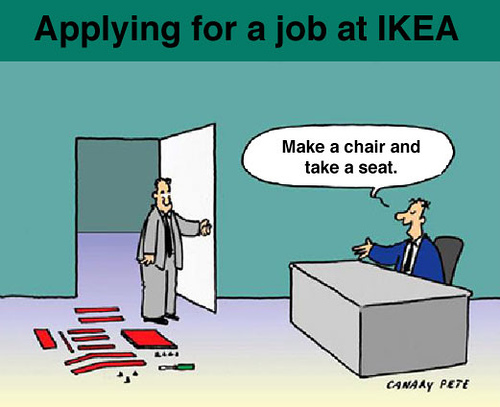
\includegraphics[scale=0.5]{IKEAInterview.jpg}
%\caption{iPhone game using a gyroscope sensor}
\end{figure}
Profound understanding of the target group helps in the process of creating a useful concept. It will be an answer to the users specific needs and wishes. Dividing the target group into different group categorizations - segments, gives a possibility to understand the chosen subjects deeper and hopefully it leads to a better project. The prototype will be specifically designed for a segmented and generalized group of people of this project. Connecting with target group is essential since the product will be used by actual customers. It is not enough to generalize a group of people from surface observations or presumed stereotypes, since sometimes people do not act as they speak and their actual needs can vary a lot. In the target group section, detailed information about the users of IKEA will be revealed.

This project is targeting people who are IKEA customers and who recently started decorating or changing furniture or décor of their home. This section of the research includes two parts - understanding the people who has a need for the application that we develop, and IKEA's target group, the people that IKEA attracts and who are coming to shop for furniture or décor.

There are many ways to segment a target audience. Probably the most popular is Geographic or Demographic segmentation. In this case we will go deeper and have a look at Psychographics too - we want to know the specific needs of the customers which will help to design helpful app. 

\subsection{Demographics }
Demographics is segmenting that describes group of people according age, gender, family size and life cycle (examstutor.com, Demographics). This segment gives a core understanding of the audience and it helps creating other generalizations such as psychographics.

\subsubsection{What is IKEA targeted customer's age ?}
Checking IKEA's report, public documentations, websites -  it is not clear to see what age-range people IKEA is trying to attract. Contacting IKEA also did not result in finding out their specific target group's age-range. According to observations and descriptions of center, IKEA's target group's age-range is really wide - there are lounges for children and considerations for disabled and old people. At "IKEA'S Accessibility Plan" (Accessibility Plan, 2013) they mention that there are consideration to accept people from children to old aged or disabled people. The report even states that the staff is trained to help people with disabilities, their equipment and even their help-animals. All IKEA shops has mini restaurants where different people of varying age can eat. They serve special menus for children, sell wine, and has a quick walk-by coffee machines. An assumption can be made that IKEA is trying to appeal to all age-ranges and has not created a clear concept design around a specific life-cycle stage (examstutor.com, Demographics) nor age range. 
However, according to two interview sessions that were done in a local IKEA center in Copenhagen, it was more clear who is shopping there. The majority of the interviewed people were young people - between 25 and 35 years of age.

\subsubsection{gender}
IKEA does not clearly mention anything about attracting either men or women to shop in public documentation (Accessibility Plan 2013) nor on their website of Ikea.dk. This was also clear to see through observation in IKEA. However it was interesting to see that at least half of the people were shopping together: in pairs, or groups of friends or family. 
\subsubsection{Social-class}
Age and statistical information of Denmark can reveal which life cycle customers of IKEA could belong to. Picture below shows "Life-cycle" stages.
\begin{figure}[H]
\centering
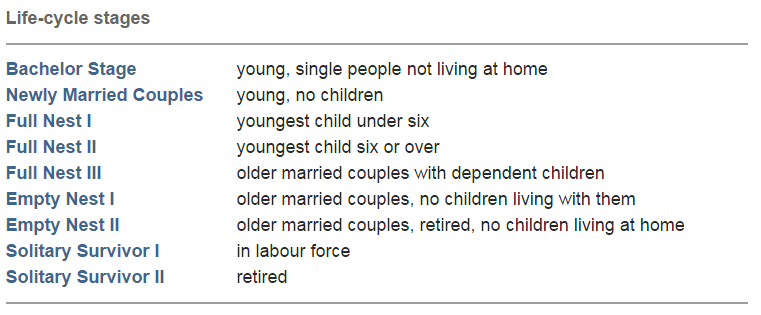
\includegraphics[scale=1]{life_cycle.png}
\caption{Picture from internet -  examtutors.com - demographics}
\end{figure}
The targets group's maximum age was set to 35, according "Statistics denmark" section "The average Dane" women has their first child at the age of 29.(Statistics Denmark 2014 - The Average Dane) This means that the targeted audience is below "Full nest II" - young families. 
 "Danish Ministry of Education" gathered statistical information of when students begin and end their bachelor (Danish Ministry of Education website - Higher education). In the picture below it is seen at which age Danish students start higher education.
\begin{figure}[H]
\centering
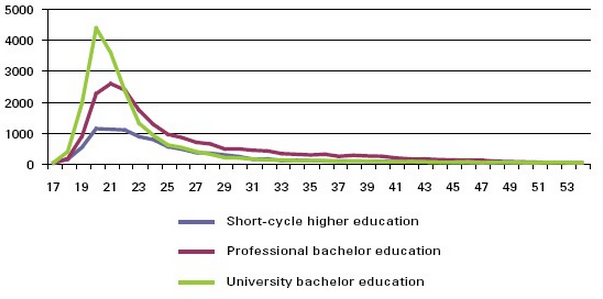
\includegraphics[scale=1]{bachelor.png}
\caption{Picture from internet - Danish Ministry of education - higher education}
\end{figure}
As it is seen in the graph above, students finish their bachelor at around the age of 25. It means that IKEA attracts people who has just finished some higher education and/or continuing master and above, since set minimum was 25.

An assumption can be made that IKEA attracts young people - Higher education students, young couples and families and of course exceptions.

\subsection{Psychographics}
Psychographic generalization segments target group according social class, lifestyle and personality characteristics. (Examstutor.com, Psychographics) It is important and relevant to understand the customer's needs, their habits and personality since it can partially answer how the app's concept can be developed. 
Since IKEA is attracting young - up to middle-aged people, it is possible to do a more accurate analysis of the social class, lifestyle and personality traits of our target group (Examstutor.com,  2015). 
\subsubsection{Economy}
Younger people generally has less money than older generations. As an example, statistical graph from US below shows the difference of income.
\begin{figure}[H]
\centering
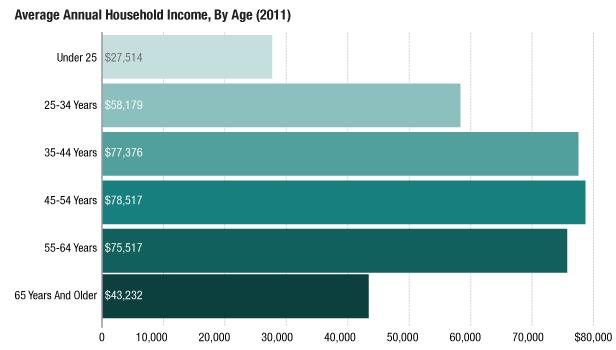
\includegraphics[scale=1]{us_income.jpg}
\caption{Picture from Internet - Income in United States}
\end{figure}

According to the "examstutor" website, social class is categorized in grade class, where IKEA's targeted customers could be defined as class C1, C2, D or E:
\begin{figure}[H]
\centering
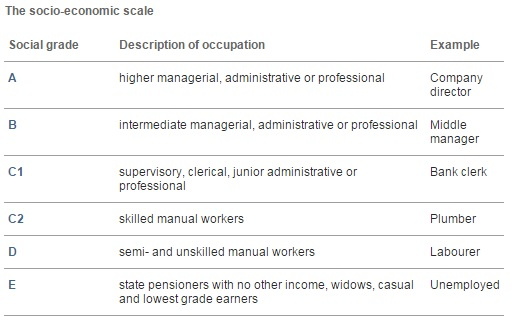
\includegraphics[scale=1]{SocialClassDiagram.jpg}
\caption{Scale of the economic classes}
\end{figure}
People in the lower socio-economic position generally have a lower income. IKEA offers low priced furniture in comparison to other Danish-market shops such as "Silvan", "ILVA" etc - it is easily seen just by visiting the websites of these shops. Therefore an assumption can be made that the younger generation are shopping at IKEA more than other people, because they care more about expenses.  

Interviewing customers confirmed that over half of the participants count their expenses. Furthermore, while interviewing employees of the shop, they noticed that the price is one of the most common topic to talk with customers about. This confirms the social class categorization mentioned above. 

\subsection{Digital knowledge}
Marc Prensky in his "Digital Natives, Digital Immigrants" (Prensky, 2001) article categorizes his understanding of target group into two segments, when it comes to understanding or learning with digital technology. He categorizes them as "digital natives" and "digital immigrants".There are few more categorizations that people use, such as "Born digital" or "Digital Settlers", so it is common to separate people into Idigital knowledge" groups.  Immigrant: Is the one who was born and grew up before the technological revolution, for example a 65 years old man who did not have all the computers and digital tools or equipment that people do now. This person only adopted the technology at a certain age or point in their life when it was needed. Digital native is the one who grew up in the technological era, where he had access for example to the Internet, computers and probably experienced one or more ways of learning in a digital environment (Prensky, 2001). However, Prensky notes that time will make everyone a "digital native", as everyone will be born in a world full of advanced technology, so old generalization terminology will not be suiting in the future. He quotes Albert Einstein - "The problems that exist in the world today cannot be solved by the level of thinking that created them." Prensky later introduces "Digital wisdom" that is a more general term but fitting in this era.(M. Prensky, 2008). This "tag" is best suited to this target group - if IKEA's customers are young students or people around 35 years of age it means that the target group is on the edge of being called both- if a person born in the 80s or 90s he/she had a chance to learn or use modern technology, depending on geographical and social class of course. That is why the terminology of "Digital wisdom" is useful - assumption can be made that most of the target group will be with digital-wisdom. Therefor most of the targeted users should not have huge problems when they start using any digital application.

\subsection{Users do plan}
Interviews with target group also gave knowledge that the users plan and prepare before going to the actual shop. Almost all of the interviewed people do some kind of measurements when buying furniture. All the interviewed people checks the website or catalogue before going to IKEA, the majority do plan before going. 

\subsection{Target group conclusion}
The target group of this project are young - middle aged IKEA customers from 25 to 35 years of age. Almost every customer has access to personal a smartphone and digital-wisdom when it comes to using its applications. The targeted people are careful with their expenses and consider the price, they also tend to know about the product before actually visiting the shop. Excluding exceptions, IKEA's customers are graduated or students who study further than bachelor, also young families and couples.




\section{User Experience Strategy}
The app that this project is aiming at developing will have a focus on the intuitive user experience. To have a focus on intuitiveness means that we must be able to understand what that implies. The dictionary defines intuitive as: 
\begin{itemize}
\item perceiving directly by intuition without rational thought, as a person or the mind.
\end{itemize}
they define the concept of intuitiveness as human perception by intuition, what then is intuition? again the dictionary will provide a relatively easy answer: 
\begin{itemize}
\item intuition\\
\begin{enumerate}
\item The act or faculty of perceiving, or apprehending by means of the senses or of the mind; cognition; understanding.
\item immediate or intuitive recognition or appreciation, as of moral, psychological, or aesthetic qualities; insight; intuition; discernment:
an artist of rare perception.
\item the result or product of perceiving, as distinguished from the act of perceiving; percept.
\item Psychology. a single unified awareness derived from sensory processes while a stimulus is present.
\end{enumerate}
\end{itemize} from this definition it is clear that the concept of intuitiveness is a human concept, more specifically a human subconscious concept. In an article from 1994 Jef Raskin\cite{JRaskin} talks about how intuitiveness comes from familiarity, while the article is quite old the observations that he makes does support the idea that intuitiveness is directly linked with the targeted users. In the article Raskin talks about an experiment that he performed, where he asks a test participant to perform a certain task with a mouse, back in 1994 the mouse was still not a tool that was commonplace and as such the test subject had no familiarity with how to work with a mouse, and required help. Raskin showed the participant how to move the mouse in the correct manner, and instantly the participant knew how it worked and didn't require any more help, because as Raskin notes: \textit{"The directional mapping of the mouse was "intuitive" because in this regard it operated just like joysticks (to say nothing of pencils) with which she} [The test participant] \textit{was familiar"}\cite{JRaskin} this observation strongly supports the idea of intuition as familiarity. With this in mind the goal of this section becomes clear: first this section will give a brief overview of the topic of user experience. Next the section will try to define what the intuitive user experience is, and lastly how does the gained knowledge translate to being used as guidelines for making an intuitive app for a mobile device.  

\subsection{Introduction to user experience }\label{UXIntro}
A study of user experience\footnote{hereafter referred to as UX} is a study of how a user feels when interacting with a system. The field encompasses a whole range of different and seemingly unrelated topics. The most known part of UX is probably the concept of usability which will be discussed later in the section, other things make up UX, such as: Design, Accessibility, System performance, Ergonomics, human factors and more concepts\cite{UXIntro}. The term user experience  was originally coined by Dr. Donald Norman, who was the first to describe the importance of user-centered design. User-centered design is a design concept that lets the users dictate(to a certain degree) what the system should contain and what form it should take.
Before user-centered design the general design process looked like:
\begin{figure}[H]
\centering
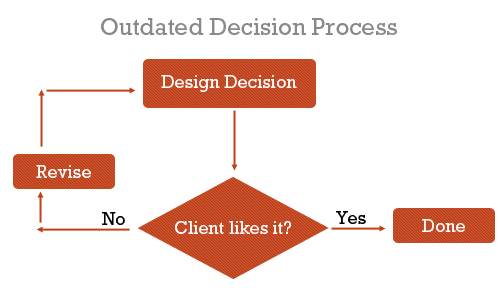
\includegraphics[scale=0.8]{OutDatedDecisionProcess.jpg}
\caption{old decision process, Jacob Gube 2010}
\end{figure}
nowhere in the design process was the users a factor, the design was simply made according to how the designers as well as the client felt it should be. making the same kind of chart for a user-centered approach would look:\\
\begin{figure}[H]
\centering
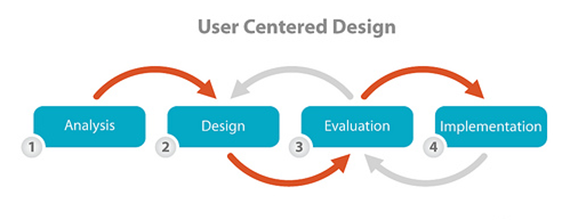
\includegraphics[scale=0.8]{UserCenteredDesign.png}
\caption{a chart of how user-centered design could function, Usabilla 2014}
\end{figure}
as this chart shows, user-centered design can be an iterative process. the grey arrow represents the user feedback, which shows that the users should be involved in the evaluation of a design.

User Experience and usability is often confused since a large portion of the guidelines for proper usability also applies to giving a good user experience. What sets the user experience apart from usability is that UX deals with the feeling of usage and usability deals with the effectiveness of usage
\todo{source for the example}An example of which could be the iBooks app for iPad.
\begin{figure}[H]
\centering
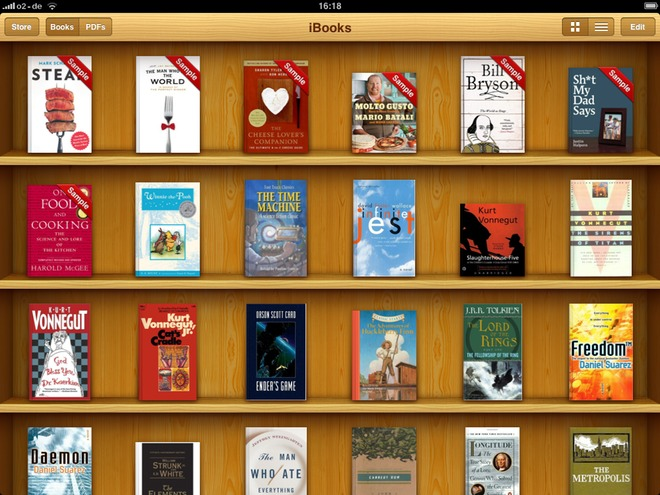
\includegraphics[scale=0.5]{iBooks.png}
\caption{Apple iBooks for comparison}
\end{figure}\todo{might need a source reference}

\begin{figure}[H]
\centering
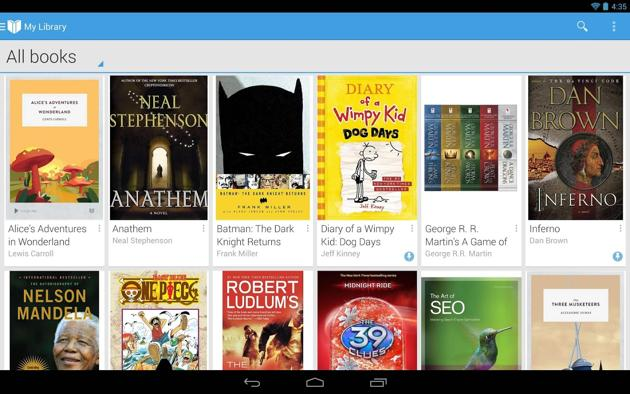
\includegraphics[scale=0.5]{GooglePlayBooks.png}
\caption{Google Play Books for comparison}
\end{figure}\todo{might need a source reference}
An application for reading and browsing E-books. The layout is simple, it provides an overview of the owned books with a visual representation of the covers which is common for such apps and as such, do not set itself apart from the state of the art when it comes to usability, however the user experience is greatly improved simply by changing the background to resemble a bookshelf, it makes the experience of logging onto IBooks resemble the experience of going into a book store or library a lot more, this approach relates to the concept of intuition as familiarity, which will be discussed in the next subsection.   



\subsection{Intuitiveness is familiarity}
as explained in the previous section \ref{UXIntro} user centered design is a main pillar of user experience, this is even more true when talking about intuition as a design concept. As Jared M. Spool mentions in his 2005 article \textit{People Intuit, not Interfaces}\cite{JaredMSpool} the article mentions that it is the users that define whether or not an interface is intuitive as the interface itself is nothing more than a collection of code. What this shows is that for an interface to be intuitive, a comprehensible knowledge about the targeted users' previous experience with similar interaction, is not only useful but absolutely crucial. the article introduces the concept of a knowledge space, which is the arbitrary space that holds all the knowledge that pertains to a given interface. 

\begin{figure}[H]
\centering
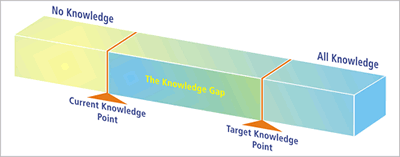
\includegraphics[scale=1]{KnowledgeSpace.png}
\caption{the knowledge space viewed as a continuous curve going from \textit{no knowledge} to \textit{all knowledge} \cite{JaredMSpool}}
\label{fig:Knowledge}
\end{figure}

As seen in figure: \ref{fig:Knowledge} there are two points of interest in the knowledge space that is the \textit{Current Knowledge Point} and the \textit{Target Knowledge Point} a brief explanation of the two points:
\begin{description}
 \item[\textbf{Current Knowledge Point}] \hfill\\
 This is the expected user knowledge which can be defined by a multitude of ways i.e. user interviews, analysis of similar apps etc. Figuring out what the current knowledge point is will enable the app to fill the knowledge gap without having to guide the user through every tiny detail. 
\item[\textbf{Target Knowledge Point}]\hfill\\
this is the amount of knowledge a user needs, to be able to use the app/programme as intended.
\item[\textbf{The Knowledge Gab}]\hfill\\
the knowledge gab is all the knowledge that the app/programme will have to provide to the user, this is usually done with a series of tutorials. 
\end{description}

He puts forth two conditions which he determines are the two conditions needed before users will classify an interface as being intuitive, these are:
\begin{itemize}
\item \textit{Both the current knowledge point and the target knowledge point are identical. When the user walks up to the design, they know everything they need to operate it and complete their objective.}
\item \textit{The current knowledge point and the target knowledge point are separate, but the user is completely unaware the design is helping them bridge the gap. The user is being trained, but in a way that seems natural.}
\end{itemize} 
Of these two conditions the latter one will probably be of more use to the project as the navigation with the gyroscope will not be a control scheme that the user necessarily  have used before. Since the end product is going to introduce an uncommon way of interacting it will be important to know which kind of interaction will feel most intuitive for the user, that is where the iterative process will enable extensive testing of different interaction models, to determine the correct approach for our users.
\subsection{ Designing intuitively  }
The topics discussed in the previous section helps define what the app has to be able to do, but besides these ideas, besides these topics the project will look at the following two structures that can help create a pleasant UX:
\begin{itemize}
\item Clear Umbrella Structure\\
\textit{"The umbrella structure is the overall structure that lays out what the product can do for you"}\cite{UXKeys} the umbrella structure is a design pattern that helps the user immediately see what the interface can do. in a 2013 article Kyrie Robinson points to Apple's central phone app as an example of a proper implementation of this structure. Further she points out that the umbrella structure can easily become an obstacle if the interface has too many features within the umbrella. 
\item  Empowering Users to Complete Tasks Faster\\
 \textit{“When a user has a good experience, one of the first things they say that they liked about it is that it was fast. Since users "equate fast with easy," }\cite{UXKeys} the app that this project will develop does not contain a wide range of features but is a relatively specialized app, while this diminishes the urgency of the app being fast, it should not be neglected. Robinson points to 6 ways of empowering the users effectiveness:
 \begin{enumerate}
 \item \textbf{Make the app work faster}\\
 this is a straight forward engineering problem, as better/less code results in a faster interface. 
 \item \textbf{Simplify your users’ work flow}\\
  this means cutting down on the amount of screens that the app employs.
 \item \textbf{Make sure your navigation is intuitive}\\\label{effectivenessP3}
 As talked about earlier intuition is related to familiarity and familiarity coupled with the umbrella structure mentioned above should be able to provide an intuitive navigation within the app.
 \item \textbf{Reduce the amount of text}\\
 in relation to the second point, if an app has a lot of text it will slow down the work flow of the user, at least in the beginning.
 \item \textbf{Examine your graphics}\\
 Robinson points to graphics as being an important part of how a user perceives an app, she urges to keep the graphics: \textit{"clean and not distracting"} 
 \item \textbf{Buttons}\\
 when making any kind of button make sure that the user never questions whether or not it is a button, further Robinson also encourages to give the buttons one word labels such as "send", "buy", "find" etc. of course the words should represent the action that the button performs.
 \end{enumerate}\cite{UXKeys} 
\end{itemize} 
these points together with the intuitiveness discussion above should enable the app to provide an intuitive user experience. 

\subsection{Usability}
According to John Wiley’s “Interaction design”, there are usability goals that worth considering when developing interactive usable system (Wiley, Interaction design, 2015). Covered usability goals are:
\begin{itemize}
\item effective to use - it is how system does what it suppose to do;
\item efficient to use - how does the system supports user while he interacts 	with it;
\item safe to use ;
\item good utility - provides with variety of functionality that user might need; 
\item easy to learn;
\item easy to remember how to use.
\end{itemize}

Wiley notes that not all of the goals are needed for most of the systems. Specific system should have specific goals. Probably most important and relevant for this application design is effectiveness and efficiency. To help user to navigate 3D environment easy system has to be with accurate response which saves time and does wanted task quickly. Fx. if user wants to view 3D object from certain angle, it is easy and fast to navigate to the point where the view angle is desired. For the beginners of such interaction with 3D environment, “easy to learn” and “easy to remember” goals would be most relevant. Don Norman in his “The Design of Everyday Things” states that there is principle of “Affordance”. (Norman, The Design of Everyday Things, 1988)  Principle is being explained as fx. Cup is affordable to being picked up; door is affordable of being opened because of it’s handle; button affords being pressed etc. So if the user is beginner, principle of affordance is extremely useful. Norman notes that there are two “affordances” real and perceived. Real is the one in real world as in examples mentioned above, and perceived is imitation of real. Fx. in this design, for beginners users especially, navigation buttons needs to look very similar to “real” navigation buttons. Fx. if user is familiar with any common video gaming console buttons, they have to be represented in a interactive software system with similarity to real one. 

Don Norman also covers other principles of usability:
\begin{itemize}
\item Visibility - how visible is the button on the screen ?
\item Feedback - what kind of feedback does the system gives to the user ?
\item Constrains - visual constraints as fx graying out some menu which is not used;
\item Mapping - layout of menus, buttons etc.;
\item Consistency - layout’s, colors, typography etc consistency through the system;
\item Affordance  - real and perceived affordance, covered above.
\end{itemize}
(Norman, The Design of Everyday Things, 1988)

Like with usability goals not all of the principles of usability needs to be in one system. However, in this case, design of the program can include all mentioned principles. Fx, if the 3D navigation system is controlled by the buttons on the screen, they need to be visible, give some sort of feedback when pressed, mapped out with consistency rules and visualized with “affordance” principle. 

\subsubsection{Mobile Usability}

Since the design of this system is meant to be on a mobile platform, there are certain aspect to consider. Some users might have limited mobility or problems with manual dexterity (e.g. has a case of Tetraplegia) - it will cause higher error rates with the interaction (Wiley, Interaction design, 2015). Even small aspects like person’s bigger fingers can cause troubles while using mobile phone and especially while interaction needs precision. This problem is mentioned in many articles, reports, researches as fx. in “The Generalized Perceived Input Point Model and How to Double Touch Accuracy by Extracting Fingerprints” where they introduce possible solution to this problem. Since the focus of this project is not solving such problems, deep analysis will not be done. However, some considerations might be done, as fx. using Norman’s principle of “feedback”. Buttons pressed on screen can change color or size, mobile device could use some sensors to indicate that action was achieved, as vernation, blinking flash etc. It is especially useful since most smartphones using on-screen touch buttons and physical sensation of touching the button is not existing.  In that case, user who did not register if he successfully completed wanted action, mobile device would help and give feedback using its sensors. Feedback is also useful to people who do not put lots of attention to their interaction accuracy, fx pressing somewhere around button area and not on it. Feedback would help user to know if action was successful. 
In general, it is important to consider minorities and helping user effectively understand their efficiency of actions. Since this non-traditional interaction method can be used by many people as was discovered in analysis of target group, product needs to be optimized to at least fit majority of the users. 

\subsubsection{conclusion}

Considering Norman’s and Wiley’s mentioned usability goals and principles it is possible to create an useful application. Usability goals of effectiveness and efficiency, will be achieved by using all covered principles. Principles will be used in creation of visual elements and coding. Having goals as easy to learn and remember, will help user with digital knowledge to narrow knowledge gap while using app first time. Solution to that is to create interactive navigation using affordance principle and visual familiarity.




\section{Interaction Design}
\todo{needs intro ease-in}
A very important part when developing the application to fit a pleasurable user experience is to make sure that it works as flawless as possible, and there are no misinterpretations when using the product. For the product that is going to be developed, the “traditional” interaction methods do not cover the functionalities that are needed to cover our initial concept needs. To assure that the alternative interaction is integrated in a convenient manner, knowledge about different sensors and possible combination of two or more to make more intelligent outcomes should be established.
\subsection{Traditional interaction methods and their replacement}
As technology evolves, new ways of interacting with computational devices are constantly built. With that, people’s needs also change. The transition from the classical buttons on a cellphone to a touchscreen has made new ways of interaction possible - the delimitation of physical buttons made it available to have any customised graphical interfaces on the screen possible. This made life easier for casual tasks - like zooming a photo using two fingers as multi-touch input, which is much more intuitive than the classical button alternative.
Soon enough non-traditional sensors started finding their place in smartphones - the implementation of these sensors in the smartphone allowed new forms of interaction, such as video calling, flashlight and screen orientation, followed by more interesting unusual uses - application developers started making instrument tuners (GStrings), barcode scanners, radiation detectors (GammaPix), pulse detectors (Instant Heart Rate), light intensity meters (Light Meter) and countless other applications that use the sensors to their favour in a non-traditional manner. However, we will only focus on sensors that support our problem area, which points to the ones that can work with 3d environment - the relevant ones for this project are the gyroscope, accelerometer and magnetometer. In section 2.3.2 \todo{need to reference Sensors section, idk how to do it} possible sensors and combinations of them that are considered to be used to achieve a functioning prototype will be discussed. %\begin{itemize}
%\item mention immersion
%\item if sensors are used well - sharpness achieved. beneficial for imitating %feeling of reality
%\item conclusion (non-traditional)
%\item what sensors we are going to use and why
%\end{itemize}

\subsection{Mobile Usability}
According to the Journal of Interaction Science (http://www.journalofinteractionscience.com/content/1/1/1) \todo{needs to be made into a reference}, mobile usability is measured by these three attributes: effectiveness, efficiency and satisfaction. These attributes may not always be achieved with traditional interaction methods – because they are limited to visual feedback dependent on touch interaction with the device (which, for instance, will not be able to utilize a sense of 3d placement of the device in its environment). It has also been shown that it might conflict with the users interaction, if the user has limited mobility (e.g. has a case of Tetraplegia) – it will cause higher error rates with the interaction (especially with complex applications that have smaller buttons). This project will focus on utilizing the use of non-traditional interaction methods to focus on enhancing user experience by using interactional input means that are not considered traditional.

As we are aiming for a better user experience, and one of the factors is the previous experience the user has had involving the task, a proper approach would be to guide the user through the switching process between interaction methods. E.g. if a task would normally be performed with traditional gestures, the user should be intuitively guided on how to do it in an alternative way. On the other hand, users that have no prior experience with the task or similar apps, should be able to discover what they need easily. Although, context of use is not considered often (according to the same article, less than 10\% of the taken studies took it into consideration), as opposed to previously made point.

\subsection{Sensors}
\todo{needs an introduction}
\subsubsection*{The Accelerometer}
The accelerometer is capable of detecting the force and the movement in a three-dimensional space. This feature is most commonly used to adjust the display to match the position that the device is held in by the user (Chong, 2015??). If the accelerometer is rotated at the center of the system, however, it will not detect the movement. Accelerometer, along with other sensors is commonly used in the augmented reality concepts.
\subsubsection*{The Gyroscope}
A gyroscope is a device that uses Earth’s gravity to help determine orientation. Its design consists of a freely-rotating disk called a rotor, mounted onto a spinning axis in the center of a larger and more stable wheel. As the axis turns, the rotor remains stationary to indicate the central gravitational pull, and thus which way is “down.”(Ryan Goodrich, 2013). Gyroscope, in comparison to magnetometer and accelerometer, is the physically largest and most expensive sensor, so the possible limitations in the smart devices in-built Gyroscopes have to be considered.
%http://issuu.com/eeweb/docs/01-2015_embedded_developer_2_pages/30?e=7607911/11184384

\begin{figure}[H]
\centering
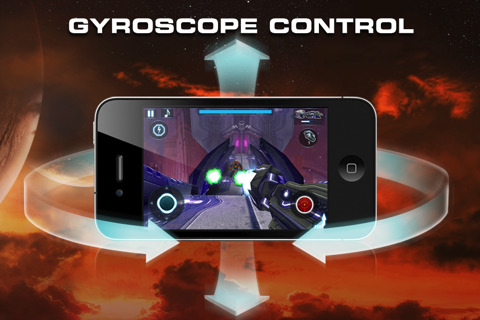
\includegraphics[scale=0.5]{GyroscopeApp.jpg}
\caption{iPhone game using a gyroscope sensor}
\end{figure}

\subsubsection*{The Magnetometer}
The magnetometer can be combined with an accelerometer (to complement in measuring the gravity) to get the input of the 3d orientation the phone is being held in. It can be useful in determining the absolute orientation of directions in the North/East/South/West plane. The issue with the magnetometer is that magnetic interference can disturb its flow, making the device output unpredictable results.
%http://www.sensorplatforms.com/understanding-smart-phone-sensor-performance-magnetometer-2/

\begin{figure}[H]
\centering
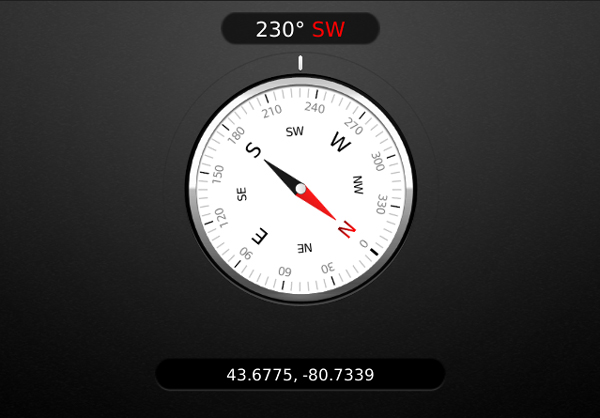
\includegraphics[scale=0.5]{MagnetometerApp.jpg}
\caption{a simple compass app that establishes the magnetometer sensor}
\end{figure}

\subsubsection*{Combined Sensors (6-axis approach)}
Combining accelerometer and gyroscope allows measurement of 6 orientations on X, Y and Z axis, allowing the apps to calculate placement of the device in the 3D environment more accurately.
\todo{these 2 subsections need merging into 1}
\subsubsection*{9-axis approach}
Accelerometer, magnetometer, gyroscope could be all combined together for even more valuable user experience. For instance - enabling an online feature with more precise positioning in relation to other users could be considered. The data gathered from accelerometer, magnetometer and gyroscope can accurately position the artefact in the world, including the changes in position and rotation. On top of that, multiple sensors could fill individual sensors blind spots. 
%http://issuu.com/eeweb/docs/01-2015_embedded_developer_2_pages/30?e=7607911/11184384
%picture!!!

\begin{figure}[H]
\begin{subfigure}{.5\textwidth}
  \centering
  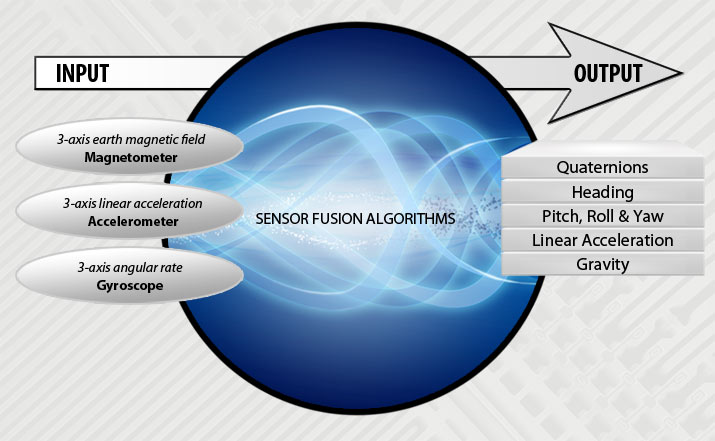
\includegraphics[width=.9\linewidth]{Sensors.jpg}
\end{subfigure}%
\begin{subfigure}{.5\textwidth}
  \centering
  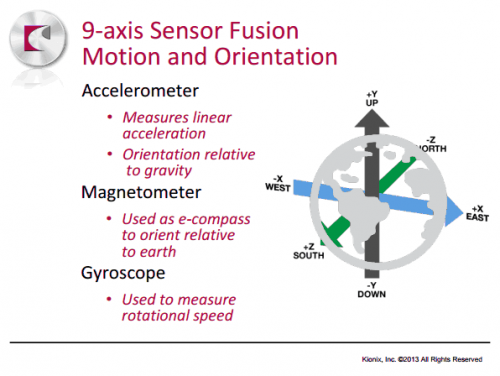
\includegraphics[width=.9\linewidth]{Sensors2.png}
\end{subfigure}
\caption{uses of sensors}
\end{figure}


\subsection{Conclusion}
After gaining more knowledge it can be seen that there is a variety of options how to use sensors in apps. Whether it is all of them together or using only few of them, it is needed to take all the options into consideration. As the project theme mentions it, the project has to be with non-traditional user interface, meaning that this project should aim for more complex or more “interesting” choices regarding sensors or user input. This means that we will go for more complex options, regarding sensors, in this case it will be 9-axis sensor fusion, combining accelerometer, gyroscope and magnetometer, as this will provide us with most accurate measurements in this project.



\section{Graphical Design}
When you dive into the ocean of possibilities that is design, there are many factors to be considered. What color palette should you choose? And which fonts goes best together. How do you find your way through mixing the right colors and fonts? And how does this affect the way your design is being perceived? 

\subsubsection{Colors}

Colours are not just colours when you are designing a brand, an app or a website. Colours are perceived in various ways and is a big part of how your design is coming  across to the user. %find a source to back this up.
But first things first, let's have a look at what colours consists of.

There are to primary colours. Additive and subtractive. Additive is used on screens as it gives away light and subtractive is used for e.g. book covers as it reflects light. \cite{Colour}
These are also known as RGB(Red, blue and green) and CMYK(Cyan, magenta and yellow).
In additive colours white is colours mixed together where black is the absence of colour. In subtractive white is the absence of colour and black all the colours mixed together. 
Since subtractive colour do not fully absorb light a fourth element has been added, hence the K in CMYK. K stand for 'key' which essentially is black.\cite{Colour}

The colour wheel can helps us see which colours are complimentary, adjacent and triadic. 
\begin{figure}[H]
\centering
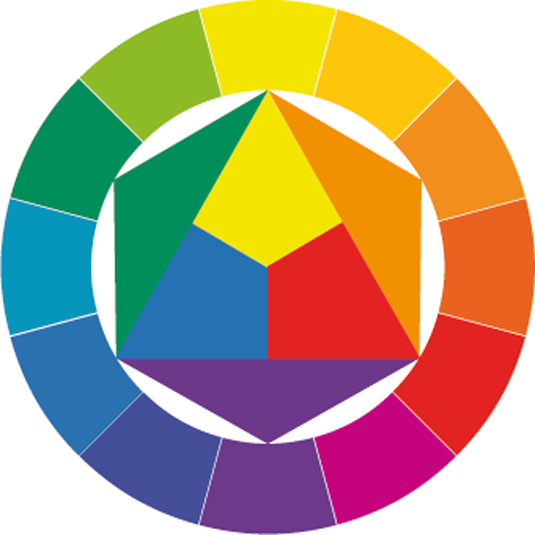
\includegraphics[scale=0.25]{wheel.png}
\caption{The colour wheel. \cite{Colour}}
\end{figure}

Colours are defined by hue, saturation and brightness. 
Using a colour gamut you can see all the different shades available. As you will discover, the RGB is much more limited than CMYK. This is because there is a limit to how much a screen is able to show. 

It is important to remember that when choosing the colour palette for a design that how we perceive colour is very different. Also, colours can change according to what you put it next to. Yellow might look different next to grey than it will next to purple for instances. \cite{Colour}

When it comes to color psychology the truth is, it is too dependent on personal experience. There is no one right answer to which color falls into what mood. \cite{ColorMeaning}
There is, however, many studies conducted on this matter. 
One study shows that 90\% of people make snap judgement based on colour alone. \cite{ColorMeaning} Another study shows that an intend of purchasing is linked with how a brand is perceived i.e. what kind of "personality" does the brand have?\cite{ColorMeaning}

\begin{figure}[H]
\centering

\includegraphics[scale=0.125]{color-emotion.jpg}
\caption{Overall image of how colours are generally percieved. \cite{ColorMeaning}}
\end{figure}

But all in all, the concept you are working with is key. Almost every study shows that it is greatly more important to choose a colour that shows the personality of your product than picking a stereotype colour. \cite{ColorMeaning} %what kind of personality does our app have? should it be inspirational?

Lastly, colour preferences differ between genders. Women prefer soft colours and tints while men prefer bright colours and shades. \cite{ColorMeaning} %Is our target group a mix or mostly female?

So how does one find the best way to coordinate different colours? Research indicates that the isolation effect is very useful.

\begin{figure}[H]
\centering
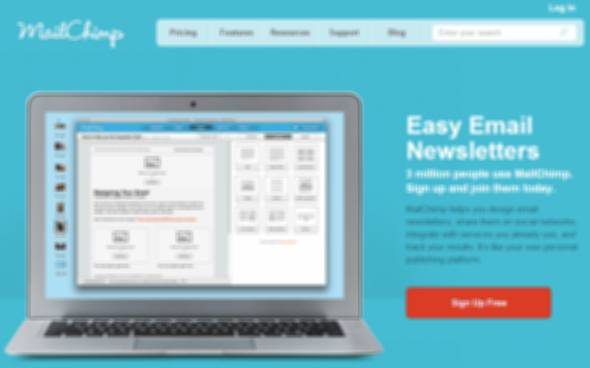
\includegraphics[scale=0.5]{isolation_effect.png}
\caption{"The sign-up button stands out because it's like a red "island" in a sea of blue." \cite{ColorMeaning}}
\end{figure}

Using the isolation effect will help the user have a more efficient experience because the most important feature e.g. a "sign up here" button, stands out. \cite{ColorMeaning} (See fig. 2.13)
Research suggests that a colour scheme that consists of analogues colors and combine it with a accent complimentary color or a tertiary color is preferred among users. \cite{ColorMeaning} %how can we use this

\subsubsection{Rythm, Balance and proportions}
Something about rhythm, balance and proportions. \cite{DesignPrinciple} %is this relevant for mobile design?

\subsubsection{Fonts}
The most popular combinations of fonts is sans serif and a serif body type. \cite{TypeComb}

Dan Mayer has created a set of guidelines to choosing a font and typeface. This consist of 5 simple rules that will make the art of choosing the right font a little easier. First thing Dan mentions is that picking a font is like picking out an outfit for the day. Appropriateness is key, although you might have some favourites that you love to use. As he says "While appropriateness isn't a sexy concept, it's the acid test that should guide our choice of font." \cite{Font}

There is a huge list of fonts to choose from. Mayer suggests that we only look at 5 key groups. 

\begin{figure}[H]
\centering

\includegraphics[scale=0.5]{type-mash.jpg}
\caption{Mayer's five groups of fonts. \cite{Font}}
\end{figure}

\begin{itemize}

\item
Geometric Sans
\\
Geometric sans is a "less is more" typeface; it is minimalistic.

"At their best, Geometric Sans are clear, objective, modern, universal; at their worst, cold, impersonal, boring. A classic Geometric Sans is like a beautifully designed airport: it's impressive, modern and useful, but we have to think twice about whether or not we'd like to live there." \cite{Font} %how do I cite this properly?

\item
Humanist Sans
\\
These Sans faces are based on hand writing. Even though some of them look clean and modern they still have a human touch. One one hand it manages to both be clear and modern but also human and empathic. One the other hand it might come across as wish-wash and and fake. \cite{Font}

\item
Old Style
\\
These are the oldest typefaces there are, hence the name. 
They are classic and traditional which can be a good or bad thing given the context. 

\item
Transitional and Modern
\\
These typefaces emerged as type designers experimented with more geometric sharp and virtuosic typefaces. 
These can seem strong, dynamic and stylish but at their worst too baroque and to stodgy. \cite{Font} 

\item
Slab Serif
\\
Slab serif is hard to generalize. It goes in many different directions and can both seem hard (Rockwell) but also friendly (Archer). As Mayer says " .. their distinctive blocky serifs function something like a pair of horn-rimmed glasses: they add a distinctive wrinkle to anything, but can easily become overly conspicuous in the wrong surroundings." \cite{Font}
\end{itemize}

Third principle - The principle of decisive contrast. When combining typefaces either go with the exact same or make a big contrast. The official name for this is Correspondence and Contrast. As the name suggests, it means that you either stay with the same typeface(correspondence) or you do something completely different(contrasting).\cite{Font}
There is no general rule to decide how to fonts go well together, they just do. But a general rule of thumb can be to choose two fonts that have one thing in common, like x-height or stroke, but are different in all other aspects. 

"A little can go a long way" is the fourth rule. In short, this teaches us that when you need something with personality only use it in a small amount. E.g. use a fun font for a headline and combine it with another more simple font for the main text. 

Mayers fifth rule is that there is no rule - the best way of finding a great fit is to try a lot of different styles. \cite{Font}

To sum up, do not overdress your text and always keep it simple. Combining a maximum of two fonts should hit the spot.\cite{TypeComb} %do we have a lot of text in our app? Is fonts relevant?

\subsection{Design Patterns}
%what is the purpose of this - also rewrite it!
Two of the things people often complaint about in applications is a confusing interface design and poor navigation. \cite{Pattern} This can be prevented by using design patterns. 
First, let's look at navigation. There are two ways to make navigating through an app easier. Persistent and transient. Persistent navigation is your list menus and your tab menus or menu structures if you will. Transient navigation has to be revealed through a tab action or the likes.\cite{Pattern}
Does the user need to see the menu at all times? If not, you can use an off-canvas solution like the side bar. 
It has become more and more popular to use off canvas methods. \cite{Pattern} This helps the app hold more information but without being confusing e.g. If all your information has to go on one page. 
You don't want to put too much text into one page or have a simple form take up several pages. A sign in for example should only be one page. A way to not get an over lapping look is by using vertical labels instead of horizontal. \cite{Pattern} Or you could have the horizontal labels where the text disappears as soon as the user starts typing, but you risk that the user forgets what they should fill in.\cite{Pattern} 
Some apps, like Instagram, shows the "sign in" and "sign up" option all the way through the tutorial. This also insures that the user do not have to go through a whole tutorial if they don’t need it. 
Another important form is the "search" form. This should be very short. It is a good idea to offer a filter option like "saved searches". There are several kinds of searches. 

Explicit search is the most standard search option and is pretty straight forward. But you can still give it a little extra. E.g. When the user chooses the search bar but haven't typed anything in yet you could give them some options in a list e.g. have a "scan" option at the top, latest searches, saved searches etc. \cite{Pattern}

Implicit search will give the user something they didn't search for and what they might not know they needed. E.g. Search for coupons when you enter your local grocery store and give an alert if there is anything useful. This will enhance the user experience as well. \cite{Pattern}

Scoped searches is searching for something more specific. You can choose to search in different categories to minimize the results and not get a result of 1500 different chairs if you are looking for one specific chair. \cite{Pattern}

Lastly there is the dynamic search or dynamic filtering. This is used to minimize choices in set lists like in music library. This is however only good with small data sets.\cite{Pattern}

There are many more patterns and anti-patterns to discover. \cite{Pattern}

Keeping these patterns in mind there are still many things to consider. 
First of all, remember the size of the screen that you are designing for. Avoid using big scaled photos and put to much information at one page. This will make it look cluttered and make it less intuitive. \cite{Sardo}
In short, make everything as clean and simple as possible. 

When designing your layout it is, once again, key to keep everything simple and streamlined. 
Follow the general rules, left-to-right and top-to-bottom. Make sure the most important feature is in the top left corner where the user will look first.\cite{Sardo}

Be careful when choosing a font type. You cant control the devices fonts and thus try to pick an common type font.  \cite{Sardo} To make the text easy to read make sure that the contrast between text and background is present. Either black and white or a light coloured background with dark text. \cite{Sardo}

Last but not least; colours. Make sure that the colours are bright enough and that the contrast is sufficient since the weather can affect the UX. \cite{Sardo}



\section{State of the Art }
Def: State of the art
\textit{ State of the art is the level of knowledge and development achieved in a technique,science, etc, esp at present }
\newline
This section will be an analysis of a number of applications that all focus on designing a room or a set of rooms. The previous sections have provided the necessary framework for doing the analysis. Specifically the analysis will cover:

\begin{itemize}
\item The familiarity the of the different aspects of the apps.\\
what parts of the app have been seen in other apps or in real life. 
\item The knowledge space for the app\\
here the analysis will try to determine if the app succesfully bridges the knowledge gap talked about in ux section ref: fig. \ref{fig:Knowledge}.
\item The graphical design: Color, overall layout. Farver, fonts og sådan overall lauout
\item The different interaction methods that is used. 
\end{itemize}
 Finally the end of this section will sum up the trends noted and will give a overview of what aspects the different applications have lacked behind with and what aspects this project could aim to improve. 

\subsection{Ikea Kitchen Planner}
In this application customers can create accurate measurements of their own kitchen and place the furniture from IKEAs catalogue. It is possible to do different wall measurements, add wallpapers to walls, apply different ceiling and floor covers, add windows and doors. Users can view the layout from top-down view and later see how the furnished layout looks in 3D perspective.

IKEAs web application for designing kitchens is used mainly in actual IKEA stores. This could indicate that users need help using this application It is used as a tool with focus on efficiency and not so much an app you would use at home for interior design. Most of the people that were asked in the initial interview also confirmed that they do not use this application. Some of the participants are familiar with the app and have tried it but do not use it. 

When you first enter the app there are no immediate help or tutorial. There is, however, two places in the app where it is possible to get help yourself. Very reasonable layout going from left to right and top to bottom.  There is a lot of easy-recognizable buttons which helps the user experience along. 
It is very slow though which highly affects the usability. The app uses click and drag.

\begin{figure}[H]
\centering
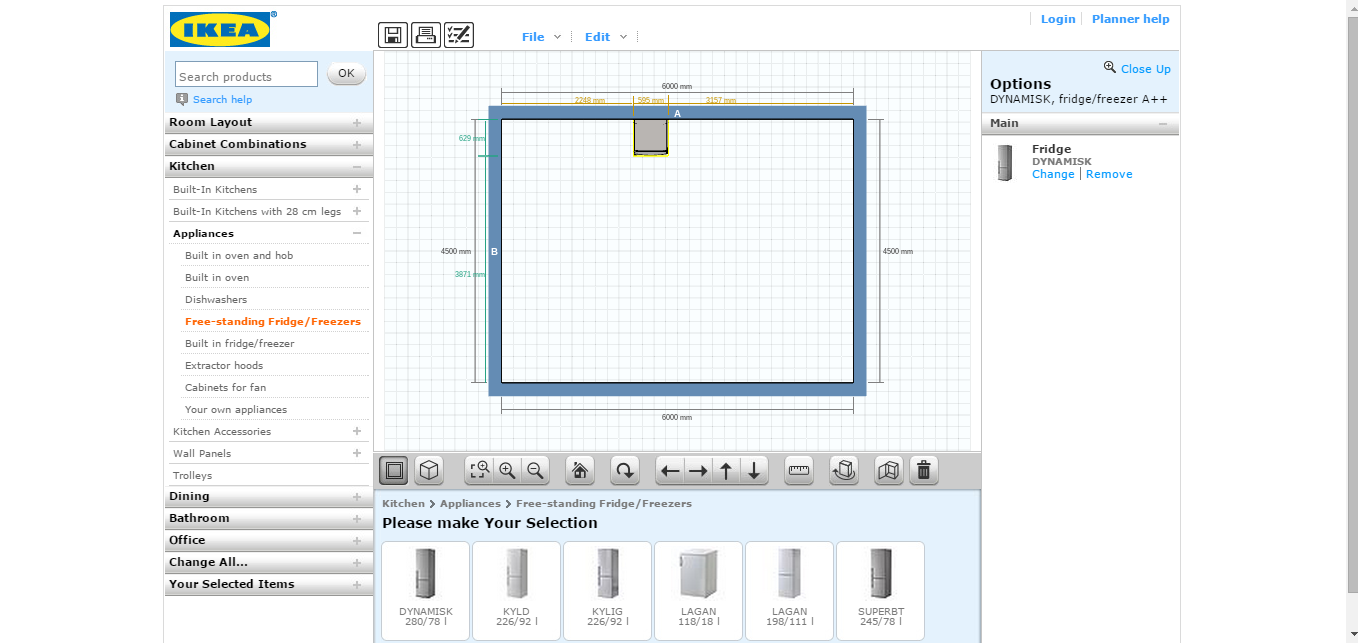
\includegraphics[scale=0.25]{IKEAPlanner.png}
\caption{IKEAs kitchen planner webapplication in 2D mode.}
\end{figure}

The app is grey and clinical but again, it is a practical tool for IKEA customers to visualize a kitchen. 
The application offers plenty of useful features and can be used to give a grasp of how peoples homes would look like prior to buying the actual items, however, it is rarely used by IKEAs customers. The problem could be that the application is hard to use, leading to long time spans used to build the desired kitchen design. A solution to this possible problem could be to create an application that is more intuitive and takes less time to achieve the users needs.

\subsection{HomeDesign3D}
This mobile application is made for interior design. It has most of the basic features; building rooms, placing furniture, windows and doors. The user can then switch to a 3D view. Here there is two settings to choose from - a joystick where you use both thumbs to move around the house, or arrows where you can view the room by moving your finger around and use the arrows to move from room to room. From the 3D view you can paint the walls and change flooring.

\begin{figure}[H]
\centering
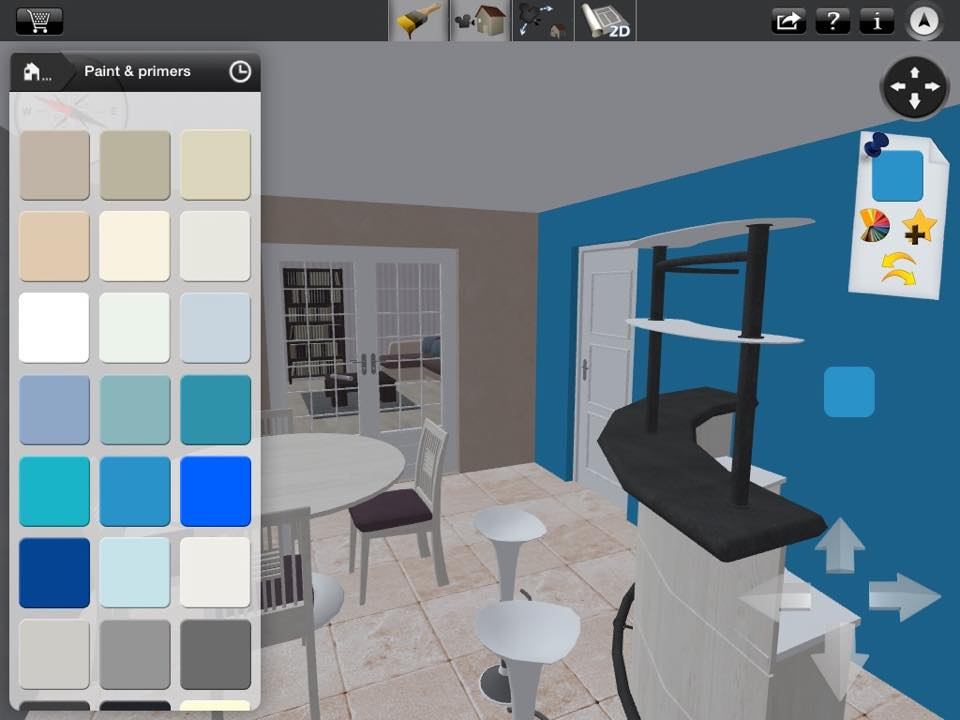
\includegraphics[scale=0.25]{HomeDesign3D.jpg}
\caption{HomeDesign3D application. Painting walls.}
\end{figure}

When you first enter the app you are faced with the option of buying the full version. This is actually the start of a long tutorial. It is very hard to notice though, since the points at the bottom that indicates that you can swipe is covered by a commercial. It is very unlikely that the user will find this help from the beginning and therefore will properly “go back” to the menu. The tutorial is easy to understand but very long. It has both pictures and text. It looks messy because of the background and the hand drawn hand that shows how to do the different thing. It is not very consistent in matters of graphical design. 
You can find this app later on in the menu. 
The next step is the design. There is apparently no start menu or the likes. 

The icons are easy recognizable.  
The layout looks very cluttered. There is the big commercial at the bottom and the menu bar in the top. 
The mix of the black bars and buttons with the beige background does not go very well together. The fact that the background is textured as a wall as well does not help the graphical aspect of this app. 

\subsection{AutoDesks HomeStyler}
This app is autodesks attempt at making an interior design app. the app does not provide a user  guide  from when you open up the app, this is opposed to the idea about bridging the knowledge gap with tutorials. The app does however provide a guide for users, once they are actually designing their room, but if the user is not able to get to this point then they are stuck. The overall look of the app is reminiscent of the flat design pattern as seen in Windows 8, this makes the app feel very modern. it also makes the app look very exclusive. However during the main activity of the app the design does not exactly match the look when browsing the catalogue, this leads to the app lacking consistency. 

\begin{figure}[H]
\centering
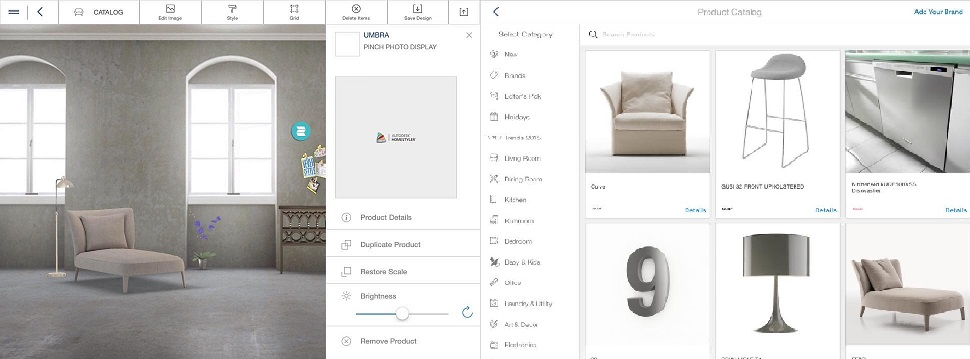
\includegraphics[scale=0.5]{AutodeskCombined.jpg}
\caption{Homestylers lack of consistency. Right: The design of the catalogue. Left: The design of the actual room planning feature.}
\end{figure}

The apps button design also seem to be focused on bigger screens than a smartphone. The 
big button at the top, labelled Redesign is a good example of both the isolation effect mentioned in \ref{idas 
section}\todo{fix reference to reference to Idas section on the isolation effect} and also the button follows the principle of having the buttons be labelled with a single word \ref{robinsonUX}.
The interaction in the app is primarily clicks, with some multi touch functions for the more 
advanced functions such as resizing, moving and rotating furniture. These functions are explained the first time the user is using them and then never again.

\subsection{Planner5D}

Planner5D is an application made both for web and mobile. The web is however better executed than the mobile version. This app allows you to build rooms and place furniture, windows etc. 

\begin{figure}[H]
\centering
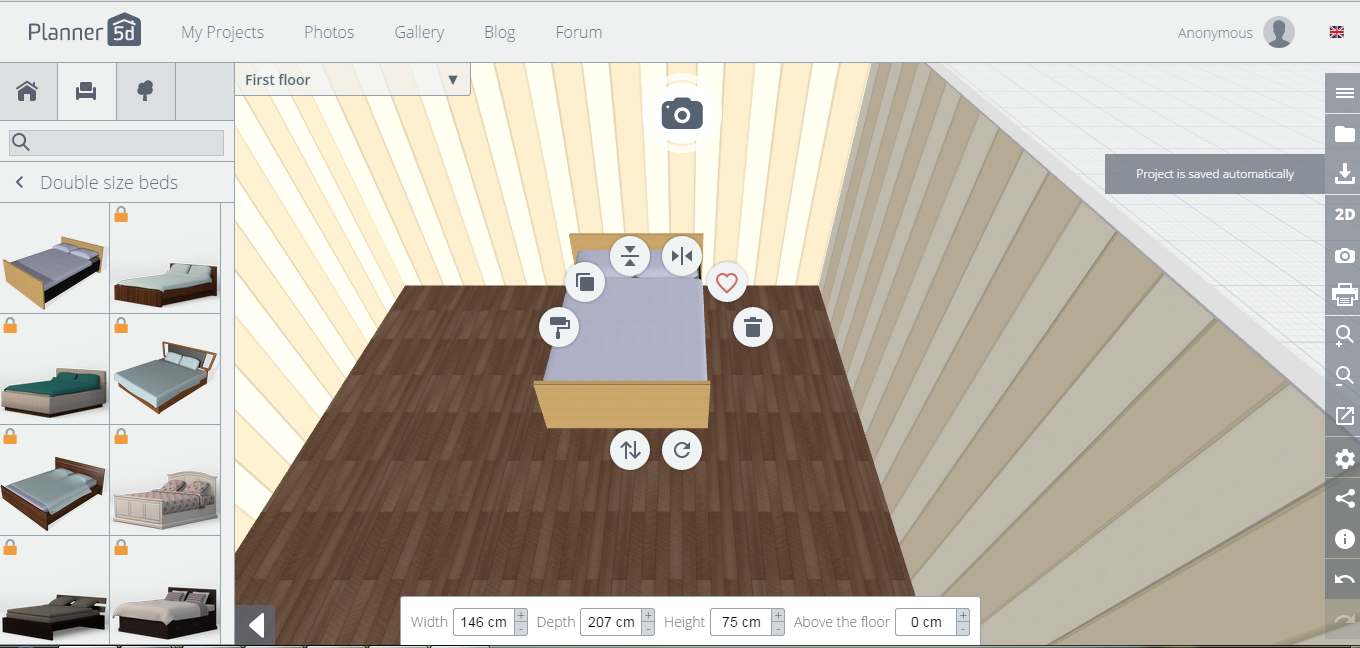
\includegraphics[scale=0.25]{Planner5D.png}
\caption{Planner5D, placing furniture.}
\end{figure}

Start screen gives a nice tutorial but is primarily composed of text. The knowledge gap is very tiny, close to nothing.
The menu bars is well divided into four sections.
The menu on the left is very apple like in its graphical feedback. Besides this there is a toolbox which is nicely divided by category, a bar at the top for social/profile aspects and lastly a menu that appears when you have placed a piece of furniture in the room; this is only in icons and no text hovers over this which makes it unclear what the different buttons do since the icons are not very familiar. A lot of focus on user friendliness. 
The app uses mainly point and click with drag.

The graphic design is very minimalistic and modern. The different features has been nicely placed which puts the focus on your own design. 
The furniture interaction does not match the real life movements of the user.

\subsection{Conclusion}

To sum up, the applications uses a variety of controls. Most of them uses click and drag, some a bit of multi touch and one has two options; joystick or buttons. 
In general the apps seem to have a different focus, therefore a different outcome. Some are very user friendly and meant as a practical tool where as others are more focused on design. 

What we can conclude from this, is that only two in four uses non-traditional interaction to their advance. Only one has a tutorial that is not text based and provides the optimal knowledge at the first encounter or makes the UI so intuitive or familiar that a tutorial is unnecessary.

Since this application does not aim to creating an interior design tool this will not be concluded upon.
\section{Design Requirements}\label{DesignRequirements}
There are two main focus areas: familiarity and knowledge-gap. This chapter will discuss these two aspects and establish specific design requirements. 
The goal for the prototype is to define which way to control the 3D virtual environment is the most familiar one for the user. As mentioned in the User Experience chapter (\ref{FamiliaritySection})\todo{fix this label!!}, familiarity is very related to intuitiveness.
To minimize the knowledge gap for the users with digital knowledge, two conditions from the knowledge gap (section \ref{intuitiveConditions}) will be upheld through the concept of familiarity. The users are expected to understand the controls and use them with a small amount of practice. Based on that, several design requirements need to be established. In general, navigation has to give a positive user experience and the user has to be in a state of "flow". 

\subsubsection{Technical requirements}
\begin{itemize}
	\item Graphical User Interface
		\begin{itemize}
		\item Controllers
			\begin{itemize}
				\item The controllers have to be familiar to the user and the buttons needs to stand out by using perceived affordance, isolation, visibility, mapping and consistency principles [ref 1 -Usability][ref 2 - Graphical design]\todo{Fix this label}
				\item Consider graphical element placement and sizes as the navigation is for mobile platforms
			\end{itemize}
		\end{itemize}
	\item Software engineering
		\begin{itemize}
			\item Controls has to be responsive and effective [ref 3 - UX Conclusion]
			\item Controls has to give effective feedback [ref 4 - UX Conclusion]
		\end{itemize}	
\todo{Fix this label}
\subsubsection{Concept requirements}
	\item Navigation
		\begin{itemize}
		 	\item Navigation has to be familiar for the user \\
The navigation should either relate to controls the users have used before or relate directly to the real world.	
		 	\item Make use of the gyroscope in context of familiarity
		 	\item 3D navigation test level\\
The level has to help reveal each control scheme's efficiency and effectiveness [Ref - Usability]\todo{Fix this label}
The level also has to challenge the user to a certain 	degree in order to be able to compare the different designs. The level must also make it clear to the user what the objective is and how they should achieve the goal, in order to measure the effectiveness of the 	controls. The colour scheme of the level should help put the focus on the objective \ref {somethings}\todo{Fix this label} rather than the surroundings.
				\end{itemize}
\end{itemize}

\section{Conclusion}

\subsection{Final problem statement}
\textit{How does non-traditional interaction using the concept of familiarity help minimize the knowledge gap for users with digital wisdom, for navigating in a 3D environment?}

1\begin{thebibliography}{9}
%\bibitem{powerGen}
%	Breeze, Paul.
%	\textit{Power Generation Technologies}
%	2nd edition,
%	Newnes,
%	2014,
%	\textit{[ISBN:978-0-08-098330-1]}

\bibitem{Chong}
  Chong, J. 
  \textit{Expanding the Functionality of Mobile Applications with Magnetic Gyroscopes} 
  In Kionix,
  2015.
  
\bibitem{Graphic}
	\textit{Building Mobile User Experiences}
	Giorgio Sardo
	\url{https://msdn.microsoft.com/en-us/expression/cc964299.aspx}
	\textit{[Last Accessed on 23-03-2015]}
	
\bibitem{Sardo}
  Georgio Sardo,
  \url{https://msdn.microsoft.com/en-us/expression/cc964299.aspx}
  

\bibitem{Pattern}
	Neil, Theresa.
	\textit{Mobile Design Pattern Gallery}
	2nd edition,
	O'Reilly Media, Inc.,
	2014.
	\textit{[978-1-4493-6363-5]}
		
\bibitem{MobileUsability}
	Jakob Nielsen, Raluca Budui
	Web ISBN-13: 978-0-13-312215-2
	Print ISBN-13: 978-0-321-88448-0
	
\bibitem{TypeComb}
	\textit{Best Practices of Combining Typefaces}
	Douglas Bonneville
	\url{http://www.smashingmagazine.com/2010/11/04/best-practices-of-combining-typefaces/}
	\textit{[Last Accessed on 23-03-2015]}
	
\bibitem{DesignPrinciple}
	\textit{The Principles of Design}
	Joshua David McClurg-Genevese
	\url{http://www.digital-web.com/articles/principles_of_design/}
	\textit{[Last Accessed on 23-03-2015]}
	
\bibitem{Colour}
	\textit{How To Master Colour Theory}
	Sam Hampton-Smith
	\url{http://www.creativebloq.com/colour/colour-theory-11121290}
	\textit{[Last Accessed on 23-03-2015]}
	
\bibitem{Font}
	\textit{“What Font Should I Use?”: Five Principles for Choosing and Using Typefaces}
	Dan Mayer
	\url{http://www.smashingmagazine.com/2010/12/14/what-font-should-i-use-five-principles-for-choosing-and-using-typefaces/}
	\textit{[Last Accessed on 23-03-2015]}
	
\bibitem{ColorMeaning}
	\textit{The Psychology of Color in Marketing and Branding}
	GREGORY CIOTTI
	\url{http://www.helpscout.net/blog/psychology-of-color/}
	\textit{[Last Accessed: 26-03-2015]}
		
	
\end{thebibliography}2013
\end{document}

